

\section{Penelitian Terkait}
\label{sec:penelitian_terkait}

Untuk membantu menyusun Tugas Akhir ini, digunakan beberapa penelitian yang pernah dilakukan sebagai sumber referensi. Referensi berikut digunakan sebagai pertimbangan dalam penyusunan desain solusi, atau untuk mengerti konteks dari tema yang dibahas.

\subsection{Socialize}

Socialize adalah sebuah aplikasi yang dibuat untuk membantu penelitian tentang aplikasi yang menerapkan konsep-konsep dari Digital Wellbeing. Dalam penelitian yang berjudul “The Race Towards Digital Wellbeing: Issues and Opportunities”, \textcite{CHI2019SOCIALIZE} meneliti aplikasi-aplikasi berbeda yang berkaitan dengan konsep Digital Wellbeing untuk menemukan fitur-fitur yang umum ditemukan.

Dari 42 aplikasi yang diteliti, ditemukan dua fungsi paling utama dari aplikasi berkonsep Digital Wellbeing adalah melacak dan memvisualisasi data penggunaan serta melakukan intervensi untuk mengurangi ketergantungan. Dalam upaya pelacakan data, 57\% aplikasi memiliki fitur menampilkan semacam visualisasi ringkasan dari penggunaan \textit{smartphone} pengguna, dan 50\% dapat menampilkan penggunaan per aplikasi. Dalam menampilkan ringkasan, aplikasi biasanya menggunakan grafik untuk memberikan visualisasi data (60\% aplikasi) atau \textit{widgets} yang lebih mudah diakses pengguna dari homescreen \textit{smartphone} (38\%).

Untuk melakukan intervensi, aplikasi-aplikasi menyediakan fitur untuk memberikan batas waktu penggunaan pada aplikasi atau disebut app timer (31\%), fitur yang memblokir akses ke aplikasi (26\%) atau masuknya notifikasi (19\%), fitur yang membatasi waktu penggunaan \textit{smartphone} (26\%) atau memblokirnya secara keseluruhan (15\%), atau fitur untuk beristirahat dari \textit{smartphone}-nya secara sementara (15\%). Sebagai fitur tambahan, beberapa aplikasi membantu pengguna dengan memberikan kutipan motivasi (12\%) atau suatu jenis penghargaan jika berhasil menyelesaikan suatu tantangan terkait Digital Wellbeing. Informasi lebih lengkap dari penemuan Roffarello dan De Russis dapat dilihat pada Gambar \ref{img:ruf_table} dan Gambar \ref{img:ruf_chart}.

\begin{figure}[h]
  \centering
  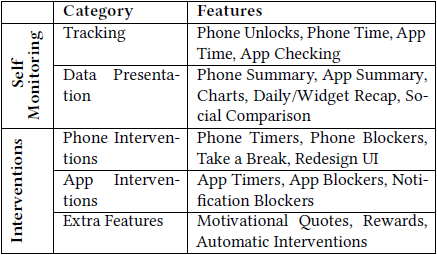
\includegraphics[width=0.5\textwidth]{chapter-2-ruf_table.png}
  \caption{Fitur-fitur umum pada aplikasi-aplikasi berkonsep Digital Wellbeing \parencite{CHI2019SOCIALIZE}}
  \label{img:ruf_table}
\end{figure}

\begin{figure}[h]
  \centering
  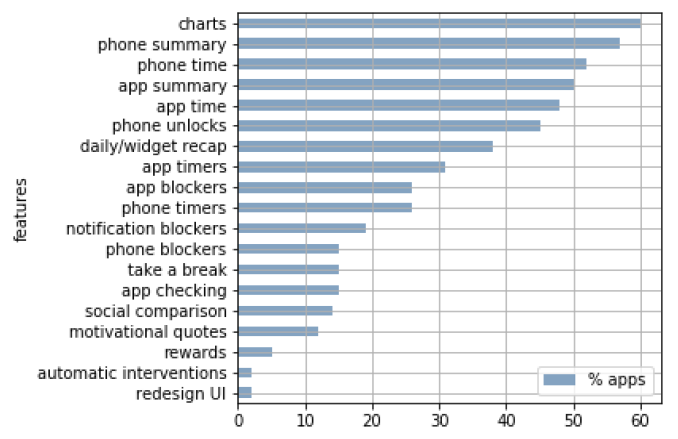
\includegraphics[width=0.7\textwidth]{chapter-2-ruf_chart.png}
  \caption{Distribusi fitur pada aplikasi-aplikasi berkonsep Digital Wellbeing \parencite{CHI2019SOCIALIZE}}
  \label{img:ruf_chart}
\end{figure}

Setelah melakukan penelitian terhadap fitur-fitur aplikasi, dilakukan pula analisis tematik terhadap 1.128 ulasan pengguna untuk aplikasi-aplikasi tersebut yang mencakup ulasan antara tahun 2015 dan 2018, baik ulasan positif maupun negatif. Hal ini dilakukan untuk mengetahui fitur apa saja yang disukai atau tidak oleh penggunanya. Roffarello dan De Russis menemukan bahwa banyak pengguna yang memang menyukai ide dari konsep Digital Wellbeing untuk memonitor dan memperbaiki kebiasaan penggunaan \textit{smartphone}, terbantu dengan mudahnya menggunakan aplikasinya. Pengguna menyukai banyaknya fitur yang tersedia, seperti pembatasan waktu dan pemblokiran akses, pelacakan dan statistik data, serta pemberian motivasi melalui penghargaan dan kutipan motivasi, dapat membantu memperbaiki kebiasaan penggunaan \textit{smartphone} atau kebiasaan lainnya secara efektif. Tak hanya itu, pengguna juga menemukan bahwa aplikasi sangat berguna untuk kasus penggunaan seperti pembatasan penggunaan \textit{smartphone} di saat belajar atau bekerja, pemantauan dan pengendalian perangkat milik anak kecil oleh orang tua, serta bantuan untuk memperbaiki jadwal tidur.

Di sisi lain, banyak pengguna yang mengeluhkan aplikasi-aplikasi kurang bersifat membatasi dan mudah untuk dikelabui, membuatnya tidak efektif dalam membatasi orang-orang yang kecanduan. Ada juga pengguna yang mengkhawatirkan tentang privasinya selama menggunakan fitur pelacakan, menilai aplikasi terasa intrusif. Selain itu, banyak ulasan pengguna yang mengeluhkan bug dan kecacatan desain hingga membuat aplikasi tidak berguna. Seluruh penemuan dirangkum menjadi kumpulan kata kunci yang dapat dilihat pada Gambar \ref{img:ruf_review}.

\begin{figure}[h]
  \centering
  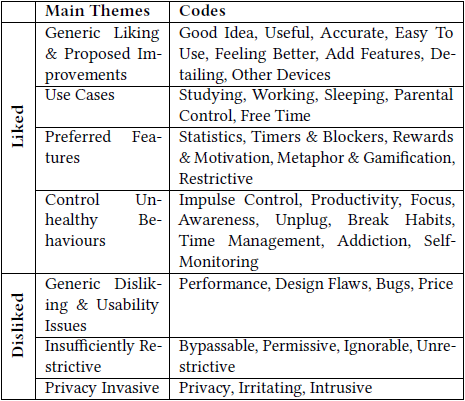
\includegraphics[width=0.5\textwidth]{chapter-2-ruf_review.png}
  \caption{Kata kunci pada analisis ulasan aplikasi-aplikasi berkonsep Digital Wellbeing \parencite{CHI2019SOCIALIZE}}
  \label{img:ruf_review}
\end{figure}

Dari analisis fitur umum dan ulasan, Roffarello dan De Russis membuat sebuah aplikasi Android bernama Socialize yang mencakup fitur-fitur paling umum dari aplikasi-aplikasi tersebut, yaitu fitur yang muncul pada setidaknya 15\% dari aplikasi-aplikasi yang dieksplorasi. Fitur-fitur yang diimplementasi dapat ditemukan pada Gambar \ref{img:ruf_fitur}, sedangkan tampilannya dapat dilihat pada Gambar \ref{img:ruf_app}. Lalu dilakukan pengujian aplikasi Socialize terhadap 38 orang untuk membandingkan penggunaan \textit{smartphone} sebelum dan sesudah memakai aplikasi. Secara kualitatif, ditemukan bahwa seluruh partisipan bersedia untuk menggunakan aplikasi Socialize lagi jika dirilis menjadi aplikasi sesungguhnya, dan memberikan masukan konstruktif tentang fitur-fiturnya. Beberapa partisipan juga antusias saat melihat statistik penggunaan \textit{smartphone}-nya. Partisipan juga mampu meningkatkan kualitas dari kebiasaan penggunaan \textit{smartphone}-nya dengan menggunakan fitur pembatasan dari Socialize. Namun di sisi lain, beberapa pengguna mengeluhkan bahwa Socialize membuat \textit{smartphone} mereka lebih boros dalam penggunaan baterai, atau mengganggu performa dari \textit{smartphone} mereka.

\begin{figure}[h]
  \centering
  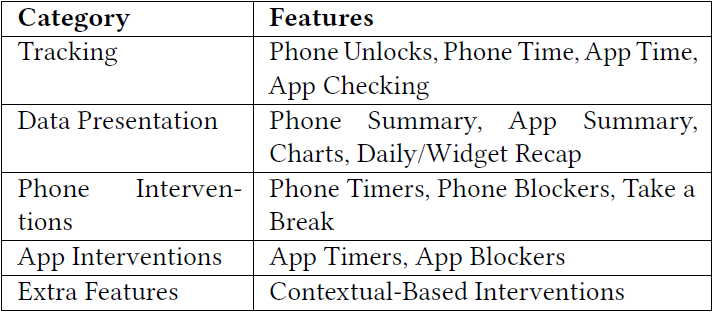
\includegraphics[width=0.55\textwidth]{chapter-2-ruf_fitur.png}
  \caption{Fitur-fitur yang diimplementasi pada aplikasi Socialize \parencite{CHI2019SOCIALIZE}}
  \label{img:ruf_fitur}
\end{figure}

\begin{figure}[h]
  \centering
  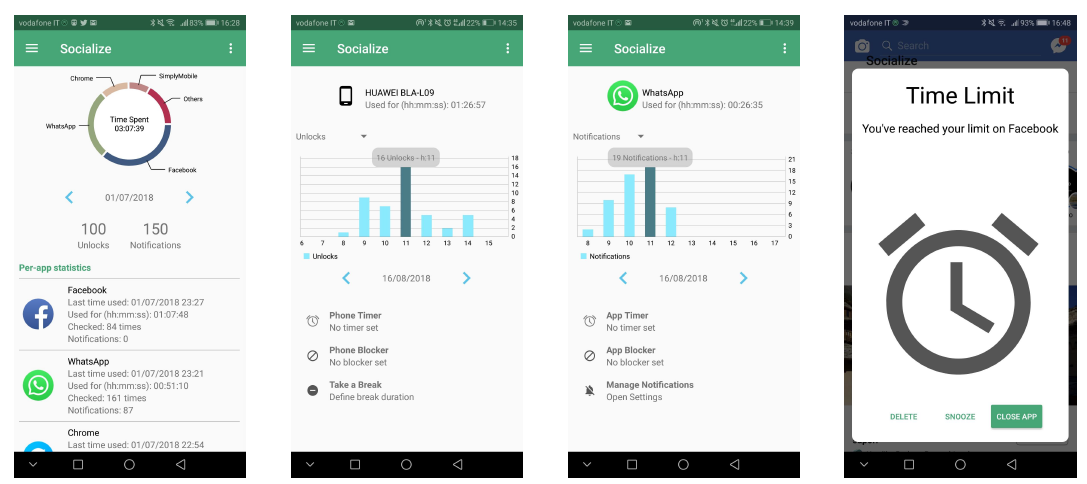
\includegraphics[width=\textwidth]{chapter-2-ruf_app.png}
  \caption{Tampilan aplikasi Socialize \parencite{CHI2019SOCIALIZE}}
  \label{img:ruf_app}
\end{figure}

Secara keseluruhan pada penelitian aplikasi Socialize, pengguna menyukai ide dari sebuah aplikasi Digital Wellbeing untuk membantu meningkatkan kualitas dari kebiasaan digitalnya. Namun solusi yang diberikan terkadang tidak cukup untuk menyelesaikan masalah yang ada. Masih perlu dibutuhkan tekad dari penggunanya untuk memanfaatkan fitur-fitur yang ada. Adapun beberapa masukan dari pengguna seperti kurang ketatnya pembatasan yang diberikan, dan diperlukannya interaksi sosial untuk membantu pengguna dalam mendapat bayangan dari kebiasaan digital yang baik. Penemuan yang cukup besar juga mengungkapkan bahwa aplikasi-aplikasi berkonsep Digital Wellbeing hanya membantu penggunanya dalam melakukan pemantauan mandiri dan menghentikan kebiasaan lama, tanpa membantu penggunanya mengembangkan kebiasaan baru yang lebih baik. Fitur yang dapat membantu hal tersebut, seperti pemberian kutipan motivasi dan penghargaan serta adanya interaksi sosial antarpengguna, cukup jarang ditemukan dari aplikasi-aplikasi Digital Wellbeing yang ada.